\documentclass[a4paper, 10pt]{amsart}

\usepackage[]{enumerate}
\usepackage[]{setspace}
\usepackage[]{libertine}
\usepackage[]{minted}
\usepackage[]{algorithm}
\usepackage[]{graphicx}
\usepackage[]{subcaption}

\usepackage[]{microtype}
\usepackage[]{inputenc}
\usepackage[]{fontenc}
\usepackage[]{caption}

\usepackage[]{hyperref}
\usepackage[]{cleveref}
\setdisplayskipstretch{3} % vertical spacing between text and math environment
\setminted{fontsize=\footnotesize}

\newcommand*{\github}[1]{\def\@github{\color{gray!70}#1}}
\newcommand{\party}[1]{\frac{d}{d #1}}
\newcommand{\mline}[1]{\mintinline{cpp}{#1}}
\newcommand{\githublogo}{\raisebox{-1pt}{
\includegraphics[height=9pt]{github}}}
\renewcommand{\v}[1]{\mathbf{#1}}

\title[Schr\"odinger equation for two electrons]{Schr\"odinger equation for
  two electrons\\
FYS3150}
\author{Ivar Haugal\o kken Stangeby\\}

\date{\today}

\begin{document}

\begin{abstract}
  In this project we wish to solve the Schr\"odinger equation for two electrons
  in a three-dimensional harmonic oscillator well. In approaching this problem
  we first wish to solve the equation for one electron, and then later expand to
  two electrons. In fact, it turns out that the only term differing in the two
  cases is the potential, hence we can develop an algorithm that runs for any
  given potential. \\
  \noindent
  All source code can be found on my GitHub page: \\

  \centering{\href{https://github.com/qTipTip/FYS3150}{\githublogo \, \color{gray!50}\textit{github.com/qTipTip}}}

\end{abstract}

\maketitle

\begin{figure}[h!]
  \centering
  
\includegraphics[width=0.8\linewidth]{ch.pdf}
  \caption*{\href{http://www.gocomics.com/calvinandhobbes/1988/01/06}{\color{gray!50} \footnotesize\textit{Shamelessly stolen from \cite{ch}}}}
\end{figure}

\tableofcontents

\section{Physical background}\footnote{This first bit is in order for me to try
to understand what I am doing, might not be as relevant for this specific
project.}
\label{sec:physical_background}
In classical mechanics, if we know the position and momentum of a particle the
system is completely determined. The analogue in quantum mechanics is the
\emph{wave-function} \( \mathbf{\Psi}(\mathbf{r}, t)\) which describes the
state of a system. If we know the wave-function we cannot obtain, and need not
obtain any more information about the system. We will later examine the
norm-squared of this wave-function, which represents the probability of finding
a particle at a given position $\v{r}$, or if you please the \emph{probability
density} of our wave function.  Denoted
\begin{equation}
  \notag
  |\Psi(\v{r})|^2 = \mathbb{P}(\v{r}).
\end{equation}
We are however typically interested in the probability of finding a particle in
some neighborhood of $\v{r}$, which is represented by $|\Psi(\v{r})|^2 dx$.  If
we have two wave functions $\Psi_1$ and $\Psi_2$ that represent two different
configurations of the same system, then we also have a set of
\textit{superpositions}, linear combinations of $\Psi_1$ and $\Psi_2$ that
represent some configuration of the system.

We typically require that the wave function is normalized, and we will later
enforce this in our implementation. This essentially means that the
integral\footnote{I have often seen the notation $\int dx |\psi(x)|^2$ used.
Why is this done, isn't this ambiguous?} over all possible positions is equal
to one:
\begin{equation}
  \notag
  \int |\psi(x)|^2 \, dx = 1.
\end{equation}
In other words, this tells us that the probability of finding a particle
somewhere is $100\%$.

\emph{Heisenberg's uncertainty principle} tells us that if we have great
certainty in the position of a particle, then we have uncertainty in the
momentum of a particle.  Any wave function $\Psi$ can be represented as a
superposition of wave functions with a well defined observable quantity, namely
wave-length or momentum. This is essentially what de Broglies` relations tells
us:
\begin{align*}
  \psi(x) &= \int \psi(x_0) \delta(x - x_0) \, dx_0 \quad \text{definite position given by the delta-function, }\\
  \psi(x) &= \frac{1}{\sqrt{2\pi}}\int \tilde{\psi}(k) e^{ikx} \, dk \quad \text{definite wave-length given by plane-waves}.
\end{align*}

\subsection{Deriving the eigenvalue problem}
\label{sub:deriving_the_eigenvalue_problem}

The Schr\"odinger equation is a partial differential equation that tells us how
a physical system evolves with time.  The general \emph{time-independent}
Schr\"odinger equation reads
\begin{equation}
  \label{eq:time_independent_eq}
  E\Psi(\v{r}) = \hat{H}\Psi(\v{r}),
\end{equation}
which we see is an eigenvalue-equation. If we set up the Hamiltonian operator
\( \hat{H} \) for our specific system, in this case one electron, this equation
then reads
\begin{equation}
  \notag
  - \frac{\hbar}{2m}\left( \frac{1}{r^2} \party{r} r^2 \party{r} - \frac{l(l+1)}{r^2}\right) R(r) + V(r)R(r) = ER(r).
\end{equation}
We are interested in the radial part \(R(r)\) of this equation.  A series of
algebraic manipulations converts this to a form we can work with, namely
\begin{equation}
  \notag
  - \frac{d^2}{d\rho^2}u(\rho) + \rho^2 u(\rho) = \lambda u(\rho).
\end{equation}
This equation can be discretized using finite-differences which leads to
\begin{equation}
  \label{eq:discrete_eq}
  -\frac{u_{i+1} - 2u_{i} + u_{i-1}}{h^2} + V_i u_i = \lambda u_i.
\end{equation}
This defines a system of equations which can be written as a single matrix
equation with a tridiagonal coefficient matrix. We can then rewrite
\cref{eq:discrete_eq} as a matrix eigenvalue problem:
\begin{equation}
  \begin{bmatrix}
    d_1 & e_1 & 0 & 0 & \ldots & 0 & 0 \\
    e_1 & d_2 & e_2 & 0 & \ldots & 0 & 0 \\
    0 & e_2 & d_3 & e_3 & 0 & \ldots & 0 \\
    \ldots & \ldots & \ldots & \ldots & \ldots & \ldots & \ldots \\
    0 & \ldots & \ldots & \ldots & \ldots & d_{n-2} & e_{n-1} \\
    0 & \ldots & \ldots & \ldots & \ldots & e_{n-1} & d_{n-1}
  \end{bmatrix}
  \begin{bmatrix}
    u_1 \\
    u_2 \\
    \vdots \\
    u_{n-2} \\
    u_{n-1}
  \end{bmatrix}
  = \lambda
  \begin{bmatrix}
    u_1 \\
    u_2 \\
    \vdots \\
    u_{n-2} \\
    u_{n-1}
  \end{bmatrix}
\end{equation}
We observe that each non-diagonal matrix element \( e_i = -1 / h^2 \) is
constant. This can now be solved using the Jacobi method which will be outlined
in following sections.

\section{Outlining the algorithm}
\label{sec:outlining_the_algorithm}

The \emph{Jacobi eigenvalue algorithm} is an algorithm for calculating the
eigenvalues and eigenvectors of a real symmetric matrix. By performing a series
of similarity transforms the matrix is transformed into an almost diagonal
matrix with the eigenvalues along the diagonal. The eigenvectors are stored
along the way.

\subsection{Mathematical derivation}
\label{sub:mathematical_derivation}

We start by first considering a two-dimensional symmetric matrix
\begin{equation}
  A = \begin{bmatrix}
    \alpha & \gamma \\
    \gamma & \beta
  \end{bmatrix}.
\end{equation}
We can then form the orthogonal matrix $R$ given by
\begin{equation}
  \notag
  R = \begin{bmatrix}
    \cos \theta && -\sin\theta \\
    \sin\theta && \cos\theta
  \end{bmatrix},
\end{equation}
which when applied to two-dimensional vector $\v{x}$ rotates it an angle
$\theta$. Letting $c = \cos\theta$ and $s = \sin\theta$ we can examine the
similarity transform $R^{-1}AR$. This transform diagonalizes $A$ given that the
off diagonals are zero. We see that
\begin{equation}
  \label{eq:givens_two}
  \notag
  R^{-1}AR = \begin{bmatrix}
    \alpha c^2 + 2\gamma cs + \beta s^2 & (\beta - \alpha)cs + \gamma(c^2 - s^2)\, \\
    \, (\beta - \alpha)cs + \gamma(c^2 - s^2) & as^2 - 2\gamma cs + \beta c^2
  \end{bmatrix},
\end{equation}
hence we need to solve $(\beta - \alpha)cs + \gamma(c^2 - s^2) = 0$ which
gives:
\begin{equation}
  \notag
  \tau = \cot 2\theta = \frac{\alpha - \beta}{2\gamma}.
\end{equation}

We can now express all the trigonometric functions in terms of $\tau$. If we let
$t = \tan \theta$, $c = \cos \theta = 1 / \sqrt{t^2 + 1}$ and $s = ct$. This in
terms yields $\cot 2\theta = 1/2 (\cot \theta - \tan \theta) = 1/2 (t^{-1} -
t)$; which gives us the quadratic equation
\begin{equation}
  \notag
  t^2 + 2\tau t - 1 = 0.
\end{equation}
Solving this equation gives us two roots. We wish to chose the \emph{smaller}
of the two roots, in order to ensure maximum numerical stability. It is better
to rotate as small an angle as possible each iteration.

We can now express the eigenvalues of $A$ in terms of $t$. The diagonalized
matrix looks like
\begin{equation}
  \notag
  R^{-1}AR = \begin{bmatrix}
    \alpha + t\gamma & 0 \\
    0 & \beta - t\gamma
  \end{bmatrix}.
\end{equation}
Solving the characteristic equation gives us the eigenvalues. For the
eigenvectors we simply perform the inverse rotation on the identity matrix $I$.

The algorithm outlined above for a $(2 \times 2)$-matrix can very easily be
extended to an $(n\times n)$-matrix case. We introduce the \emph{Givens rotation
  matrix} given by
\begin{equation}
  \label{eq:givens}
  G(i, j, \theta) = \begin{bmatrix}
    1 & \hdots & 0 &\hdots & 0 & \hdots & 0 \\
    \vdots & \ddots & \vdots & {} & \vdots & {} & \vdots \\
    0 & \hdots & c &\hdots & -s & \hdots & 0 \\
    \vdots & {} & \vdots & \ddots & \vdots & {} & \vdots \\
    0 & \hdots & s &\hdots & c & \hdots & 0 \\
    \vdots & {} & \vdots & {} & \vdots & \ddots & \vdots \\
    0 & \hdots & 0 &\hdots & 0 & \hdots & 1 \\
  \end{bmatrix},
\end{equation}
where $c = \cos(\theta)$ and $s = \sin(\theta)$. The linear map this matrix
represents is a rotation in the $(i, j)$-plane of $\theta$ radians.  The reason
for introducing this matrix is that is works in general as the matrix $R$ in
\cref{eq:givens_two} does for two dimensional cases.

Multiplying a matrix $A$ by $G^{-1}(k, l, \theta)$ from the left and by $G(k,
l, \theta)$ from the right and solving for element $a_{kl}$ and $a_{lk}$ equal
to zero yields the following set of equations:
\begin{align}
  \label{eq:difference}
  \begin{split}
  a^{\prime}_{hk} &= a^{\prime}_{kh} = ca_{hk} - sa_{hl} \\
  a^{\prime}_{hl} &= a^{\prime}_{lh} = ca_{hl} - sa_{hk} \\
  a^{\prime}_{kl} &= a^{\prime}_{lk} = (c^2 - s^2)a_{kl} + sc(a_{kk} - a_{ll}) = 0\\
  a^{\prime}_{kk} &= c^2a^{\prime}_{kk} + s^2a_{ll} - 2sca_{kl}\\
  a^{\prime}_{ll} &= s^2a^{\prime}_{kk} + c^2a_{ll} + 2sca_{kl}
  \end{split}
\end{align}

We know that this rotation preserves the eigenvalues, however --- we also wish
to keep track of the corresponding eigenvectors. However, these get changed
under a rotation. A way to remedy this is to do the corresponding rotations to
the identity matrix $I$. The columns of the transformed $I^{\prime}$ will then
correspond to the original eigenvectors of our matrix $A$.

After applying the Jacobi method to a tridiagonal matrix $A$, we are left with
the eigenvalues $\left\{ \lambda_i \right\}_{i=0}^{n}$ along the diagonal of the
transformed matrix $A'$, and we are left with the corresponding eigenvectors as
columns in our matrix $I'$.

When plotting the wave-functions, we want to examine the norm-squared of the
functions, however we require that $\int |\psi(x)|^2 dx = 1$. We therefore
normalize our eigenvectors as following:
\begin{equation}
  \notag
  \v{v}_{\lambda_i} =
  \frac{\v{v}_{\lambda_i}}{\sqrt{\int_{\rho_{\textrm{min}}}^{\rho_{\textrm{max}}}
  |\psi(x)|^2 dx}} \quad \text{ for } i = 1, \ldots, n.
\end{equation}

\subsection{Implementation}
\label{sub:implementation}

We now discuss some of the implementation specific details related to this
project. The implementation of this follow closely the implementation details
outlined in \cite[pages~217--220]{t1}, however tailored to work with the
\mline{armadillo} library.

\subsubsection{Jacobi Method}
\label{ssub:jacobi_method}

In order to perform a complete diagonalization of a matrix $A$ using the Jacobi
method we implement the  auxiliary functions \mline{rotate},
\mline{max_off_diag} and \mline{solve}.

The function \mline{rotate} performs one single rotation in the $(k, l)$-plane
in order to zero out the elements specified. The function \mline{max_off_diag}
returns the absolute value of the maximal off-diagonal element in our matrix
and returns by pointer the position $(k, l)$ of this given element.  Finally,
the function \mline{solve} performs the Jacobi rotation until we reach our max
number of iterations or the maximum off-diagonal element is sufficiently small.

\subsubsection{Unit tests}
\label{ssub:unittest}

In order to make sure that our jacobi-method does what we want it to do I
implemented a set of test-functions using the UnitTesting framework
\emph{Catch}. I wanted to ensure that my Jacobi implementation satisfied some
basic requirements.

\begin{enumerate}[i)]
  \item One rotation needed to diagonalize a $(2\times2)$-matrix
  \item The \mline{max_off_diag} method returned the correct indices as well as
    the magnitude of correct value
  \item Repeated iteration of the Jacobi method preserves orthogonality.
  \item Application to a physical system: Solving the Schr\"odinger equation for one electron and
    returning the three lowest eigenvalues exactly within some tolerance.
\end{enumerate}

\subsection{Performance}
\label{sec:performance}

There is no way of telling a-priori how many rotations the algorithm requires
in order to finish.  This is due to the fact that off-diagonal elements that
have been zeroed out earlier may get returned to a non-zero value by a
rotation. We therefore allow our program to run until all elements are
\emph{essentially zero} given some tolerance $\varepsilon$, and at most we want our program
to run for $n^3$ iterations where $n$ is our number of time steps.

The method requires an order of $(n^2 - n)/2$ comparisons in a for-loop, with a
quadratic convergence rate.

The Jacobi method --- being a very slowly converging method --- is however well
suited for parallelization due to the fact that one can implement the method
using block matrices. A numerical performance analysis of the \emph{Block
Jacobi Method} for symmetric eigenvalue problems can be found in
\cite{blockjaco}.

\section{Two electrons in a harmonic oscillator well}
\label{sec:electrons_in_a_harmonic_oscillator_well}

We now wish to examine the Schr\"odinger equation given by a two-electron wave
function $u(r_1, r_2)$.  Introducing the \emph{relative coordinate} $\v{r} =
\v{r_1} - \v{r_2}$ and the \emph{center-of-mass coordinate} $\v{R} = 1/2
(\v{r_1} + \v{r_2})$ we can --- using similar manipulations as in
\cref{sec:physical_background} --- rewrite the Schr\"odinger equation as
\begin{equation}
  \notag
  -\frac{d^2}{d\rho^2}\psi(\rho) + \omega_r^2\rho^2\psi(p) + \frac{1}{\rho} = \lambda\psi(\rho).
\end{equation}

The quantity $\omega_r$ reflects the strength of the oscillator potential, so
intuitively the stronger the oscillator potential, the less broad should the
wave-function $\psi$ look like. We see based on our results in
\cref{fig:vary_omega} that this is indeed the case. We see that the
higher $\omega_r$ we chose, the smaller $\rho_{ \textrm{max} }$ we need.

In \cref{fig:varying_frequency} we see that the quantification of

If we plot the eigenstates for the same parameters with and without
coloumb-interaction we see that the coloumb interaction constitutes a
``widening'' of the norm-squared. Ideally I should have had some plots to
display this, but time ran out.
\begin{figure}[h!]
  \centering
  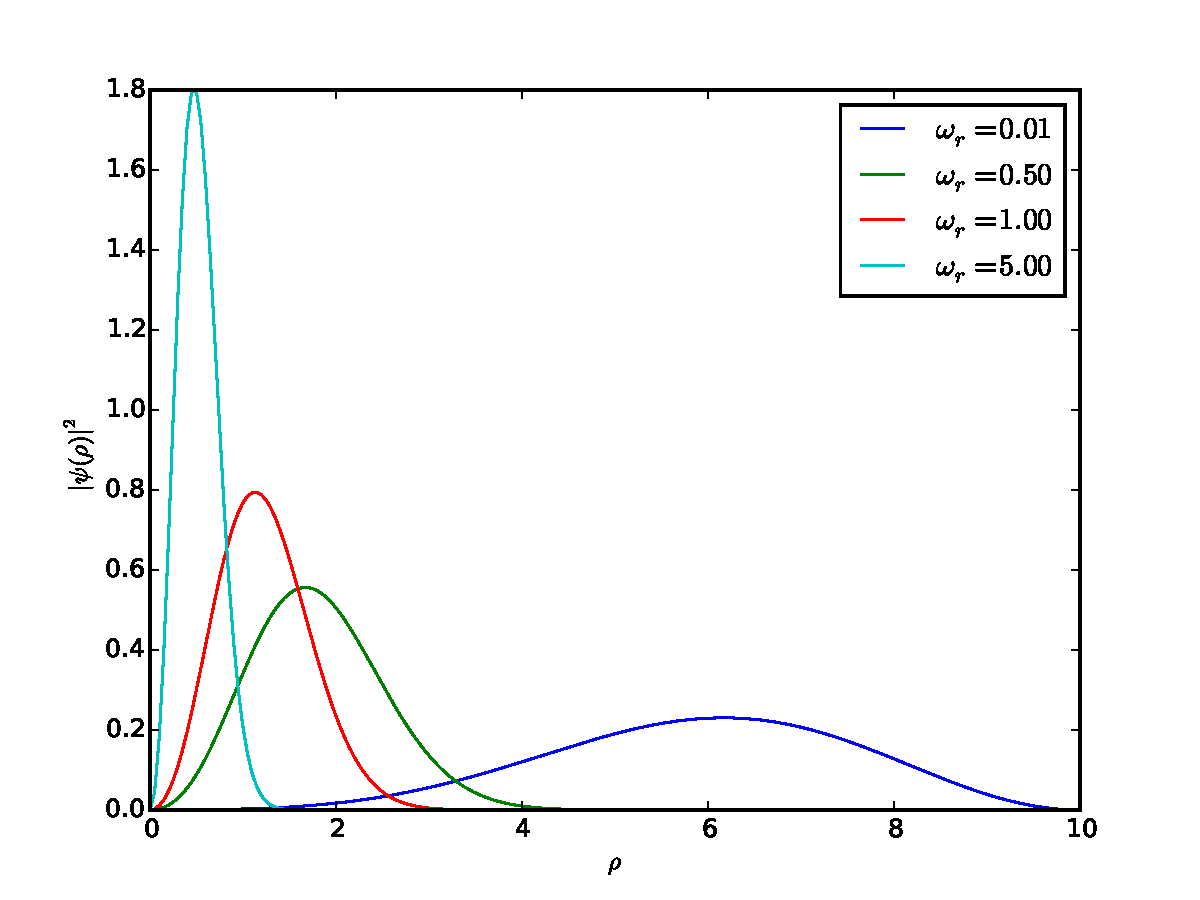
\includegraphics[width=0.6\linewidth]{./plots/schrodinger_200_10_5.pdf}
  \caption{Plotting the lowest lying eigenstate (ground state) of two electrons for various
    oscillator-frequencies $\omega_r$. We assume Coloumb-interaction. We see
    that increasing $\omega_r$ results in a more certain position closer to
    $\rho_{\textrm{min}}$ which is reasonable since $\omega_r$ represents the
    strength of the harmonic oscillator. This essentially means that the
    stronger the potential the smaller distance between the two electrons.
    Here we plot for $n = 200$ and $\rho_{\textrm{max}} = 10$.}
  \label{fig:vary_omega}
\end{figure}
\begin{figure}[h!]
  \centering
  \begin{subfigure}{0.5\textwidth}
    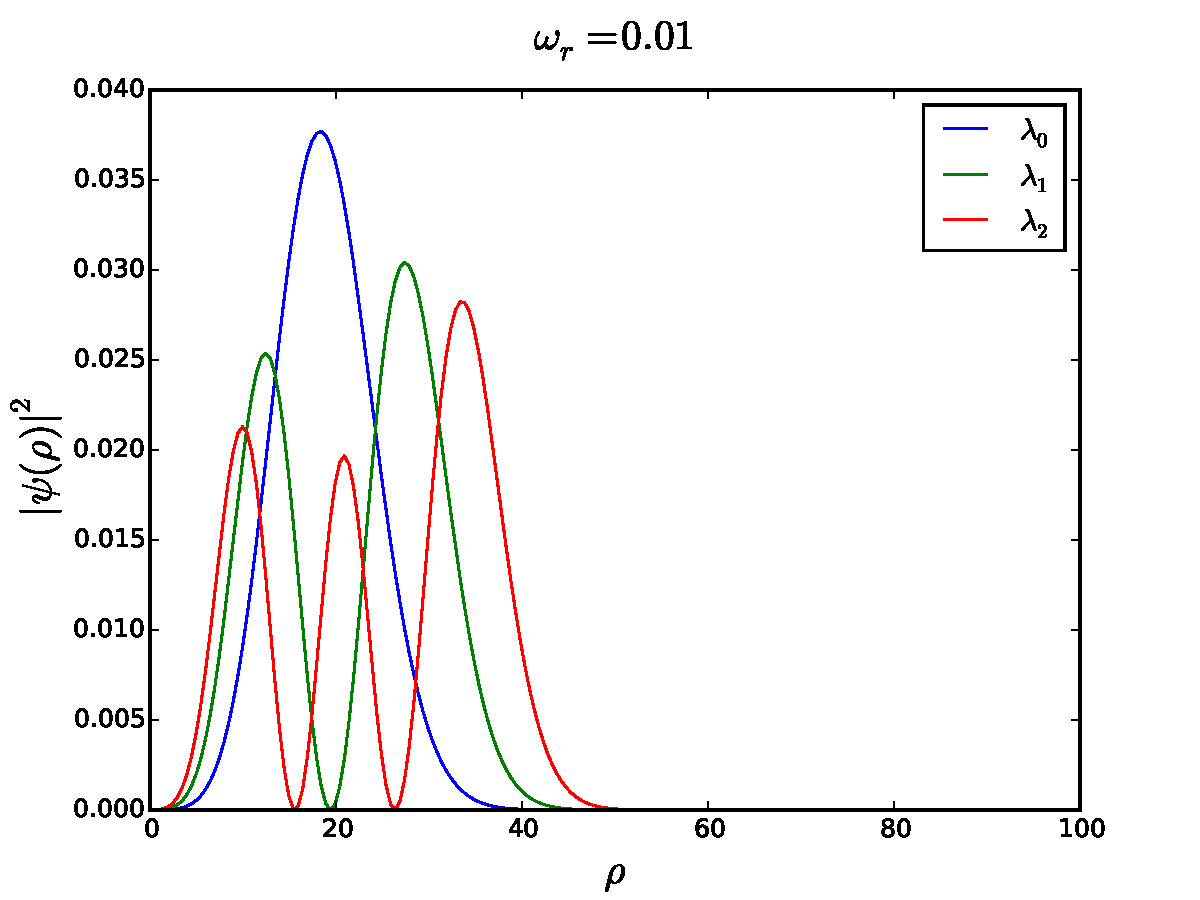
\includegraphics[width=\textwidth]{./plots/schrodinger_200_100_001.pdf}
  \end{subfigure}
  ~
  \begin{subfigure}{0.5\textwidth}
    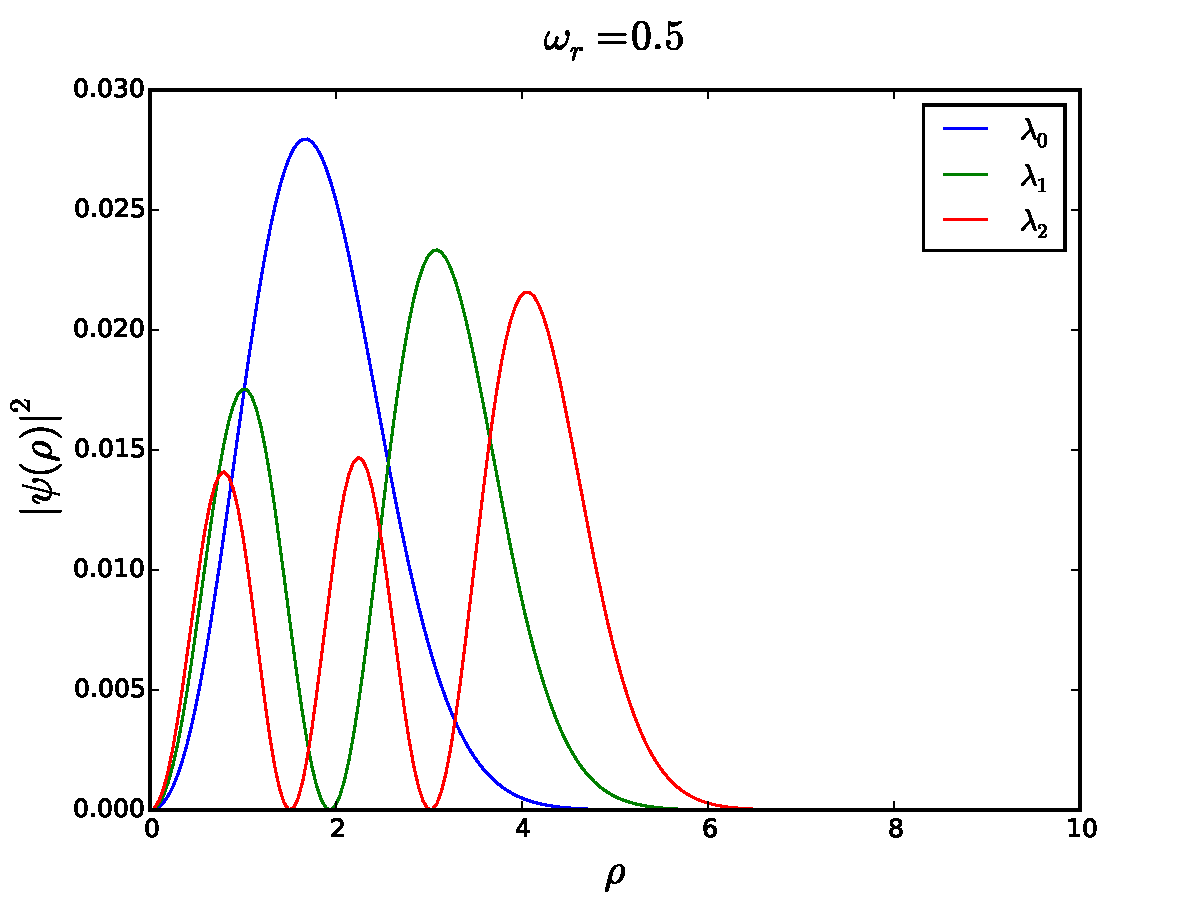
\includegraphics[width=\textwidth]{./plots/schrodinger_200_10_05.pdf}
  \end{subfigure}
  \begin{subfigure}{0.5\textwidth}
    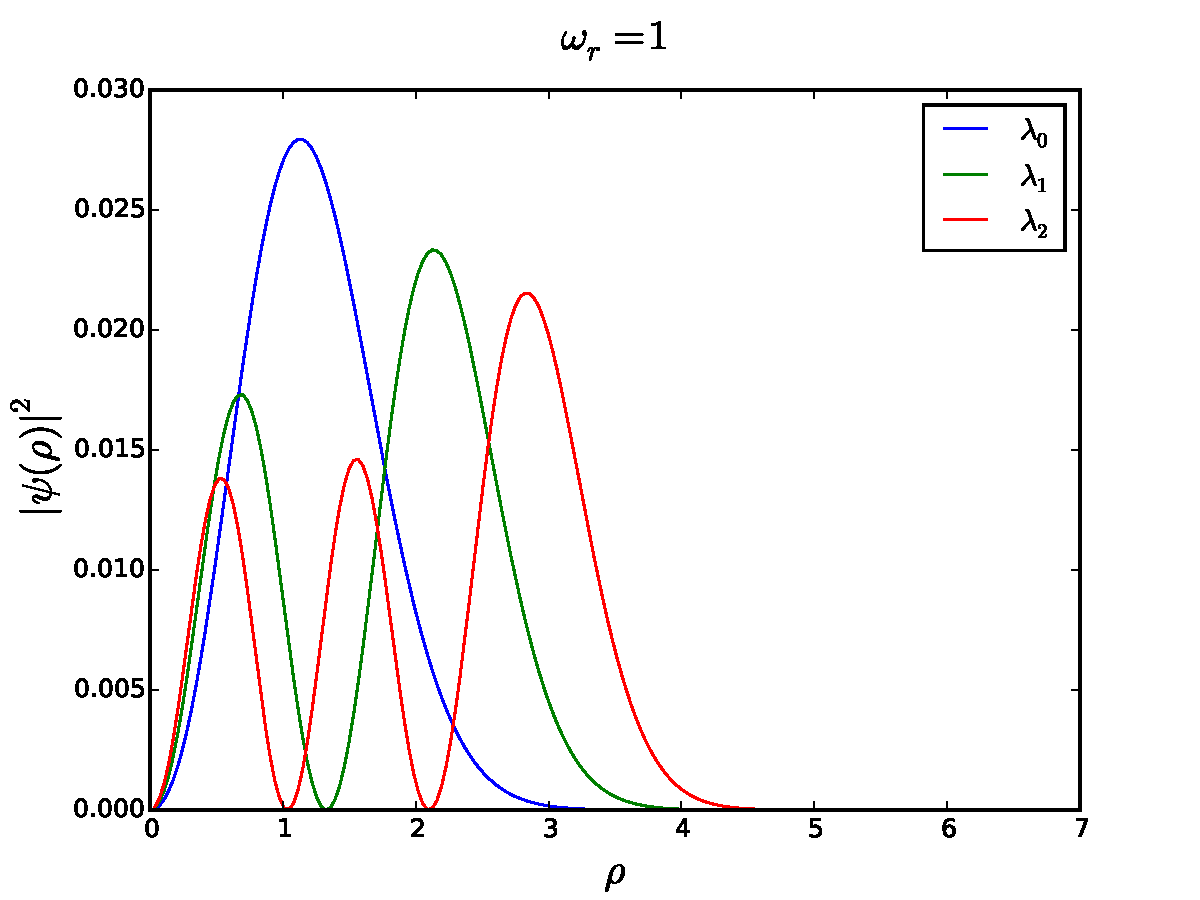
\includegraphics[width=\textwidth]{./plots/schrodinger_200_7_1.pdf}
  \end{subfigure}
  ~
  \begin{subfigure}{0.5\textwidth}
    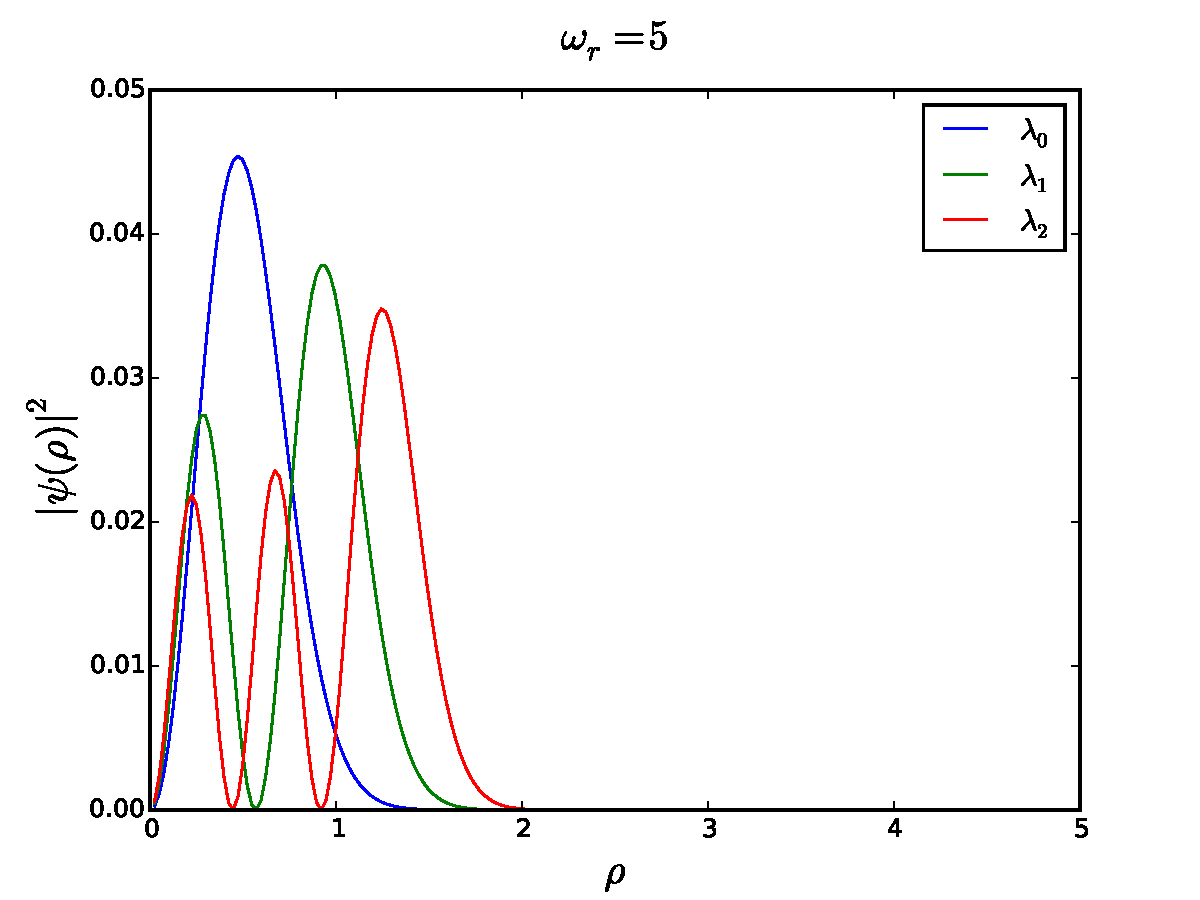
\includegraphics[width=\textwidth]{./plots/schrodinger_200_5_5.pdf}
  \end{subfigure}
  \caption{We here consider the three lowest eigenstates for each oscillator
    frequency, with $n=200$ and an appropriate $\rho_{\textrm{max}}$. We see
    that for the various oscillator frequencies the position of the electrons
    are restricted to ``bands'' of various radii from the origin. We also notice
    a small boundary-error in my program.}
  \label{fig:varying_frecquency}
\end{figure}

\clearpage
\section{Conclusion}

In this project we have examined the behaviour of two electrons with
Coloumb-interaction in a harmonic oscillator well. We reformulated the physical
problem as a discrete eigenvalue problem and solved this using the \emph{Jacobi
  Method} for diagonalizing symmetric matrices. We examine our results for
various oscillator frequencies, and the results seemed to coincide with the
predictions I made with the limited knowledge I have for quantum-physics.

A test-suite was implemented in order to verify and test the methods employed,
and I wish that I implemented the test for the non-interacting case earlier as a
test as I for a while had a bug in my potential calculatins.

No performance analysis of the algorithms were done, but I will hopefully later
have some time to compare this to the \emph{Householder's method} and the
routines included in the \mline{armadillo}-library. Since, in our case we were
working with a tridiagonal symmetric matrix, we could have written a specialized
tridiagonal solver instead which would have improved the efficiency
significantly.

\begin{thebibliography}{9}
  \bibitem{t1}
    Morten Hjort-Jensen,
    \emph{Computational Physics - Lecture Notes Fall 2015},
    Department of Physics, University of Oslo,
    August 2015
  \bibitem{t2}
  M. Taut, \emph{Two electrons in an external oscillator potential: Particular
  analytic solutions of a Coloumb correlation problem}, Laboratory of Atomic
  and Solid State Physics, Cornell University, New York, November 1993
  \bibitem{blockjaco}
    Yuusuke Takahashi, Yuusuke Hirota, Yusaku Yamamoto, \emph{Performance of
    the block Jacobi method for the symmetric eigenvalue problem on a modern
  massively parallel computer}, Algoritmy 2012
  \bibitem{ch}
    \emph{http://www.gocomics.com/calvinandhobbes/1988/01/06}, Retrieved
    October 2015
\end{thebibliography}

\end{document}
